% !TeX spellcheck = en_US
% !TeX encoding = UTF-8
% !TeX root = ../document.tex

\chapter{Model Unspecific Search in CMS}

The Model Unspecific Search in CMS (\emph{MUSiC})\cite{Pieta2012MUSiC,Papacz2014Model,Duchardt2015MUSiC} is an analysis procedure that compares observed data to the standard model expectation from Monte Carlo (MC) simulations. Unlike dedicated analyses that usually only regard a few final states, an unspecific search covers a broad spectrum of final states.
This is especially useful since some theories predict small deviations in many final states, which on their own would not be classified as significant, but in total have a scientific impact.

This chapter will focus on the MUSiC workflow. First, the motivation behind an unspecific search will be illustrated, then the three analysis steps \emph{skimming}, \emph{classification} and \emph{scanning} will be explained.

\section{Motivation}
Since a Higgs boson candidate has been discovered at the LHC\cite{Ao2015Combined}, all predicted SM particles have been observed.
Nevertheless there are many unsolved problems in modern particle physics. The most noticeable examples are the Higgs mass hierarchy problem, the matter/antimatter asymmetry, dark matter and energy and the possibility of unification theories. Various theories, such as supersymmetric extensions (SUSY), propose solutions, but they are currently lacking evidence.
Expected signatures of these models would show up in a large range of final states. For some models, narrow resonances are predicted, other result in a slight signature in the high-energy tail of the distributions.
The MUSiC analysis is sensitive to these kind of deviations.
Additionally, MUSiC can identify deviations between MC and data that originate from non-physics sources, uncovering weaknesses in the Monte Carlo simulation.

\section{Data Preprocessing}
The goal of preprocessing is to gather events from different data sources and convert them to a unified format containing only information relevant to MUSiC. AOD (analysis object data) files of observed as well as simulated events are stored on non-local parts of the computing grid, and preprocessed there. The stripped results are contained in PXL I/O files\cite{BBE+2012Development} and returned to the local computing grid.

\section{Classification}
During the classification step, events are grouped into \emph{event classes} (EC) according to their physics content in the final state. 
Missing transverse energy is treated as separate physics object. There are three  types of event classes: \emph{exclusive}, \emph{inclusive} and \emph{jet inclusive}. Final states of events in exclusive event classes contain exactly the objects indicated in the event class name. 
Events in the exclusive EC \eventclass{1e + 1MET} contain only 1 electron and missing transverse energy in the final state, but no other physics objects.
Events in the inclusive EC can contain any other objects besides the indicated ones. \eventclass{1e + 1MET + X} contains at least 1 electron and missing transverse energy. 
Additionally, there are \emph{jet inclusive} event classes (e.g. \eventclass{1e + 1MET + Njet}), that exclusively contain the mentioned objects and zero or more jets, making the analysis more robust to initial and final state radiation caused by the emission of gluons in the initial or final state.

These definitions imply that each event is contained in exactly one exclusive EC, at least one inclusive EC and at least one jet inclusive EC.

The classification algorithm automatically adjusts the possible event classes to the events actually contained in the dataset, dynamically creating new classes. 

If the dataset originates from MC simulations, some properties of the simulated processes are shifted within their uncertainties to estimate their impact on the classes. Additionally, the amount of simulated events is rescaled to match the data luminosity.

\subsection{Kinematic distributions}
Three kinematic variables are analyzed: the scalar sum of the magnitudes of all observed momenta \sumpT, the total invariant mass $\Minv = \abs{\sum p}$ and the missing transverse energy \MET.
For each event class and each kinematic variable, one histogram is filled. The histograms are created with variable bin sizes according to the detector resolution\cite[p. 52]{Papacz2014Model}. Note that the vertical axis of histograms shown in this work carries the unit "Counts per \unit{10}{\GeV}", so to get the absolute number of events in a bin, the vertical data point has to be multiplied by the width of its bin in units of \unit{10}{\GeV}.

% MUSiC/EventClassFactory/Resolutions.hh als Quelle
% Pauls Dis durchlesen
% AN: file:///T:/Temp/Downloads/AN2014_098_v5.pdf

\section{Scanning}
The scanning algorithm (\emph{scanner}) searches for the connected bin region with the most significant deviation between the data and MC yield in each histogram.

\subsection{Region Building}
For each histogram, the scanner probes all connected bin regions and calculates a \p~value for each one.

The set of connected bin regions can be defined and calculated as
\begin{equation}
R = \{(s, e) \, \forall e \in (s + m, l) \, \forall s \in (0, l-m)\}
\end{equation}
where the histogram spans the bins $0$ to $l$ and $m$ denotes a minimal number of bins per region which can be configured.

For each region, a \p~value is calculated. The region of most deviation (smallest \p) is called \emph{region of interest}.

\subsection{The \p value}
Given the number of total observed events in a region~\Ndata and an expectation~$\Nmc \pm \sigmamc$, the \p~value expresses the probability of obtaining a deviation at least as significant as the observed one, given only the standard model expectation.
Since the calculation deals with results of counting experiments, a Poisson distribution is assumed. The probability of making an observation $N$ given the Poisson mean~\Nmc is
\begin{equation}
	P(N) = \frac{e^{-\Nmc} \Nmc^N}{N!}
\end{equation}
To include observations that are more extreme than the observation, the probabilities are summed away from the expectation:
\begin{equation}
p = 
	\begin{cases} 
		\displaystyle
		\sum\limits_{N = \Ndata}^{\infty} \frac{e^{-\Nmc} \Nmc^N}{N!} &\mbox{if} \; \Ndata \geq \Nmc \\
		\displaystyle
		\sum\limits_{N = 0}^{\Ndata} \frac{e^{-\Nmc} \Nmc^N}{N!} &\mbox{if} \; \Ndata < \Nmc
	\end{cases}
\end{equation}
Since the Poisson mean is usually not exactly known, due to insufficient simulation and measurement uncertainties (e.g. luminosity), it is evaluated for multiple possible values $\theta$ which are weighted by a Gaussian distribution of width~\sigmamc around \Nmc. This final probability is called \emph{\p~value}:
\begin{equation}
p \defeq 
	\begin{cases} 
		\displaystyle
		\sum\limits_{N = \Ndata}^{\infty} C \cdot \int\limits_0^\infty \dd \theta \exp(-\frac{(\theta-\Nmc)^2}{2 \sigmamc^2}) \cdot \frac{e^{-\theta} \theta^N}{N!} &\mbox{if} \; \Ndata \geq \Nmc \\
		\displaystyle
		\sum\limits_{N = 0}^{\Ndata} C \cdot \int\limits_0^\infty \dd \theta \exp(-\frac{(\theta-\Nmc)^2}{2 \sigmamc^2}) \cdot \frac{e^{-\theta} \theta^N}{N!} &\mbox{if} \; \Ndata < \Nmc
	\end{cases}
\end{equation}
The constant $C$ denotes a normalization factor that compensates for using $0$ as the lower limit of the integral. This is necessary since the Poisson distribution with a negative expectation is not physical.

\subsection{The \ptilde value}
\label{sec:music_ptilde}
For a dedicated analysis looking at one fixed histogram region only, this \p~value would be sufficient to describe the statistical significance of the deviation. But since the scanning algorithm regards many regions to choose the most significant one from, the probability of finding a deviation somewhere in the distribution is larger than \p. This is called \emph{look elsewhere effect}.
Since MUSiC is actually interested in the global significance of the distributions deviation, the look elsewhere effect has to be corrected.
Therefor the scanning algorithm is applied multiple ($10^5$) times on randomly diced pseudo-data. For each pseudo experiment, first the expected mean $\Nmc'$ is randomly shifted from a Gaussian distribution around \Nmc, having the width of the systematic error \sigmamc. Taking this new pseudo-mean, a random Poisson number is chosen as new observed value $N_\mathrm{pseudo}$ which takes the place of \Ndata. The dicing of pseudo experiments is performed in a correlated way, the chosen deviation in units of \sigmamc is shared between all distribution in all event classes. The complete scanning algorithm is repeated for each pseudo-experiment, finding a region of interest and its \p~value.
\begin{figure}[htb]
	\centering
	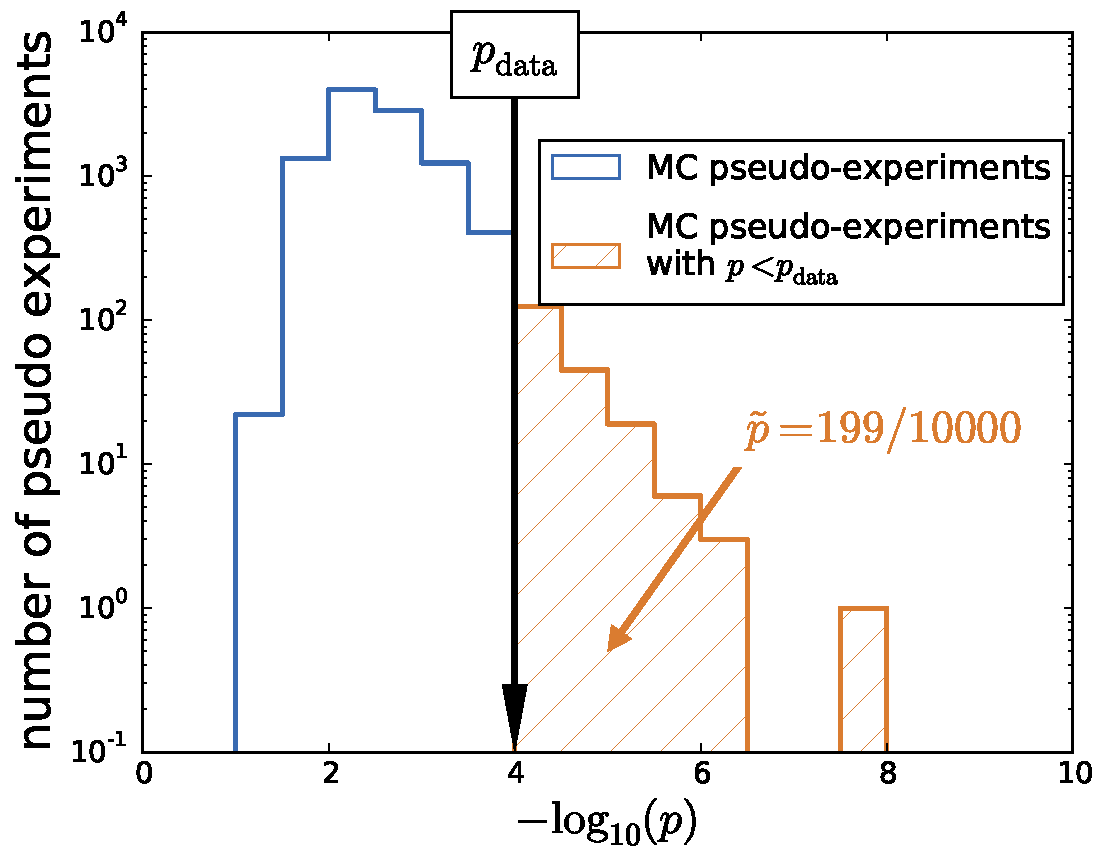
\includegraphics[width=0.6\linewidth]{ptilde_illustration.pdf}
	\caption{Illustration of a \ptilde calculation. 1000 pseudo-experiments have been conducted. The XYZ experiments on the right of $p_\mathrm{data}$ have shown a more extreme deviation somewhere in the distribution.\todo{generate graphics to insert here}}
	\label{fig:ptilde_illustration}
\end{figure}
Finally, the amount of pseudo experiments with more significant deviations than the observed one $p_\mathrm{data}$ is compared to the total amount of pseudo experiments conducted:
\begin{equation}
	\ptilde \defeq \frac{\text{number of pseudo-experiments with } \p < \p_\mathrm{data}}{\text{total number of pseudo experiments}}
\end{equation}
This calculation is illustrated in figure \ref{fig:ptilde_illustration}.
